\documentclass{beamer}

\usepackage{color}
\usepackage{amssymb}
\usepackage{rotating}
\usepackage{grffile}
\usepackage{tabularx}
\usepackage{epstopdf}

\pdfpageattr{/Group << /S /Transparency /I true /CS /DeviceRGB>>}

\setbeamertemplate{navigation symbols}{}
\usetheme{Madrid}
\usecolortheme{seahorse}

\definecolor{titlecolorr}{rgb}{0.75,0.8,0.9}
\definecolor{blockcolorr}{rgb}{0.3,0.35,0.55}
\setbeamercolor*{frametitle}{bg=titlecolorr,fg=black}
\setbeamercolor{author in head/foot}{bg=titlecolorr,fg=black}
\setbeamercolor{title in head/foot}{bg=titlecolorr,fg=black}
\setbeamercolor{title}{bg=blockcolorr,fg=white}
\setbeamercolor{block title}{bg=blockcolorr,fg=white}
\setbeamercolor{date in head/foot}{bg=titlecolorr,fg=black}

\setbeamerfont{frametitle}{size=\large}

\newcommand{\newImage}[2]{
 \begin{minipage}{#1\textwidth}
  \renewcommand{\_}{_}
  \IfFileExists{#2}
   {\includegraphics[width=1\textwidth]{#2}}
   {\centering N/A}
  \renewcommand{\_}{\textunderscore}
 \end{minipage}
}

\begin{document}

%\renewcommand{\inserttotalframenumber}{10}

\title{CxAODFramework tutorial}
\author[Daniel B\"uscher]{
\underline{Daniel B\"uscher},
David Jamin \\
for the Hbb group
}
\institute{Universit\"at Freiburg}\date{\today} 

\frame{\titlepage}

%\footnotesize
\scriptsize

\begin{frame}[fragile]
\frametitle{Outline}
\structure{Outline}
\begin{itemize}
 \item Introduction to the framework
 \item[$\Rightarrow$] Session 1: setting up the code, run a test job
 \item Details on CxAODMaker
 \item[$\Rightarrow$] Session 2: adding a variable, read the output
 \item Details on CxAODReader
 \item[$\Rightarrow$] Session 3: adding histograms, making plots
 \item How to implement a new analysis
 \item[$\Rightarrow$] Session 4: adding packages and classes
\end{itemize}
\vspace{3mm}
\structure{Links and mailing list}
\begin{itemize}
 \item This tutorial builds up on the xAOD tutorial\\
{\tiny https://twiki.cern.ch/twiki/bin/view/AtlasComputing/SoftwareTutorialxAODAnalysisInROOT }
 \item Framework TWiki\\
{\tiny https://twiki.cern.ch/twiki/bin/view/AtlasProtected/CxAODFramework}
 \item Framework repository
{\tiny https://svnweb.cern.ch/trac/atlasphys/browser/Physics/Higgs/HSG5/software/VHAnalysis/LHCRun2/CxAODFramework}
 \item HSG5 Framework mailing list: atlas-phys-higgs-hsg5Framework
\end{itemize}
\vspace{3mm}
\structure{Thanks Kristian for providing slides!}\\
{\tiny https://indico.cern.ch/event/373130/session/1/contribution/9/material/slides/0.pdf}
\end{frame}


\begin{frame}
\begin{center}
\structure{\large Introduction to the framework}
\end{center}
\end{frame}

\begin{frame}[t]
\frametitle{Run 2 workflow}
\begin{center}
 \newImage{0.99}{xAODworkflow.png}
\end{center}
\structure{Run 2 workflow}
\vspace{2mm}
\begin{itemize}
 \item adapt the new analysis scheme given by the ASG
\end{itemize}
\end{frame}

\begin{frame}[t]
\frametitle{Run 2 workflow}
\begin{center}
 \newImage{0.99}{xAODworkflowC.png}
\end{center}
\structure{Run 2 workflow}
\vspace{2mm}
\begin{itemize}
 \item adapt the new analysis scheme given by the ASG
 \item the CxAODFramework can process xAODs and DxAODs
 \item pruduce a small CxAOD (``C'' for calibrated) or a Ntuple
 \item futher tools for reading the CxAOD, filling histograms and plotting are in place
\end{itemize}
\end{frame}

% \begin{frame}
% \frametitle{Disclaimer}
% \includegraphics[page=3,width=0.99\textwidth,trim=0 0 0 140,clip]
% {../15-02-06_tutorial/Framework_Tutorial_06.02.2015.pdf}
% \end{frame}

\begin{frame}
\frametitle{Disclaimer}
This framework is developed within the VHbb analysis group (HSG5).\\
``Out of the box'' compile/runtime configurations follow the VHbb analysis!\\
\vspace{2mm}
\structure{Usage}
\begin{itemize}
 \item For running the VHbb analysis, the code is simply checked out and run. 
 \item For optimisation studies of the VHbb analysis, the code is checked out and 
modified. Optimisations are then merged into the repository.
 \item For {\color{red}other analysis}, the code is checked out and used as the base for new 
derived analysis classes. More on this later... 
\end{itemize}
\structure{“Out of the box”-contents}
\begin{itemize}
 \item The recommended calibrations are applied (CP tools).
 \item Overlap removal is performed (using official ASG tool).
 \item MET is rebuild.
 \item Object and event selections are applied.
 \item Systematic variations are run, i.e. the above steps are rerun for each variation.
 \item The output xAOD file contains the superset of objects among sys. variations, 
along with event level information. 
\end{itemize}
\end{frame}


\begin{frame}
\frametitle{Framework layout}
\structure{Framework layout}
\begin{itemize}
 \item Based on RootCore (a C++ compilation framework which depends on ROOT).
 \item Uses EventLoop (EL) and SampleHandler.
 \item Currently there are 7 RootCore packages:
\end{itemize}
\begin{center}
\scalebox{0.85}{
\newImage{0.20}{packages.pdf}
\begin{minipage}{0.05\textwidth}
\color{white} bla
\end{minipage}
\begin{minipage}{0.7\textwidth}
Main code for processing the input xAOD files, applying the calibration tools (CP tools), and writing the output CxAOD.\\ \\
Contains tools that are shared outside of the main CxAODMaker work-flow, such as object and event selection.\\ \\
Contains the code for the executables for running CxAODMaker jobs, along with any associated configuration files.\\ \\
Contains files relating to defining datasets and related information for tracking processing.\\ \\
Contains code to read CxAOD using the xAOD EDM (Event Data Model). Implements plotting style used in HSG5.\\ \\
Contains example code for producing a compact flat TTree based tuple that could be used for diagnostics or analysis.\\ \\
Contains the common TTree definition and example code to read a compact flat TTree.
\end{minipage}
}
\end{center}
\end{frame}

\begin{frame}
\frametitle{Framework layout}
\structure{Framework layout}
\begin{itemize}
 \item Based on RootCore (a C++ compilation framework which depends on ROOT).
 \item Uses EventLoop (EL) and SampleHandler.
 \item Currently there are 7 RootCore packages:
\end{itemize}
\begin{center}
\scalebox{0.85}{
\newImage{0.20}{packages.pdf}
\begin{minipage}{0.05\textwidth}
\newcommand{\blaSpace}{6.3mm}
{\Large \color{red} $\Leftarrow$} \vspace{\blaSpace} \\
{\Large \color{white} $\Leftarrow$} \vspace{\blaSpace} \\
{\Large \color{red} $\Leftarrow$} \vspace{\blaSpace} \\
{\Large \color{white} $\Leftarrow$} \vspace{\blaSpace} \\
{\Large \color{red} $\Leftarrow$} \vspace{\blaSpace} \\
{\Large \color{white} $\Leftarrow$} \vspace{\blaSpace} \\
{\Large \color{white} $\Leftarrow$} 
\end{minipage}
\begin{minipage}{0.7\textwidth}
\centering \newImage{0.6}{xAODworkflow_simple.pdf}
\end{minipage}
}
\end{center}
\end{frame}


\begin{frame}
\frametitle{CxAODMaker layout}
\begin{center}
\newImage{0.99}{classes.pdf}
\end{center}
\end{frame}



\begin{frame}
\frametitle{Calibration Tools}
List of calibration tools in framework\\
\vspace{3mm}
\begin{minipage}{0.48\textwidth}
\structure{Jets}
\begin{itemize}
 \item JetCalibrationTool
 \item JetCleaningTool
 \item JERTool
 \item JERSmearingTool
 \item BTaggingEfficiencyTool
\end{itemize}
\structure{Taus}
\begin{itemize}
 \item TauSmearingTool
 \item TauSelectionTool
 \item TauEfficiencyCorrectionsTool
\end{itemize}
\structure{Photons}
\begin{itemize}
 \item EgammaCalibrationAndSmearingTool
 \item AsgPhotonIsEMSelector
\end{itemize}
\end{minipage}
\begin{minipage}{0.48\textwidth}
\structure{Electrons}
\begin{itemize}
 \item EgammaCalibrationAndSmearingTool
 \item AsgElectronLikelihoodTool
 \item AsgElectronIsEMSelector
\end{itemize}
\structure{Muons}
\begin{itemize}
 \item MuonCalibrationAndSmearingTool
 \item MuonSelectionTool
 \item MuonEfficiencyScaleFactors
\end{itemize}
\end{minipage}\\
\vspace{3mm}
ASG analysis tools xAOD migration progress\\
https://twiki.cern.ch/twiki/bin/viewauth/AtlasProtected/ASGUserAnalysisToolsxAODMigration
\end{frame}


\begin{frame}
\frametitle{Contents of the output CxAOD}
\structure{The main guideline is to store as little as possible, which implies a trade-off}
\begin{itemize}
 \item The output file is (fairly) well organised, without too many variables creating 
confusion.
 \item Occasionally, this will also result in variables missing, and thus re-running 
of the code.
\end{itemize}
\structure{For particle-type objects}
\begin{itemize}
 \item The 4-vector is always stored. 
 \item Other chosen quantities are explicitly added by hand (with 'decorators') and stored.\\
(E.g. object scale factors, or flags for some selection criteria).
  \item The index of each particle in the input is also stored
% This enables exact comparisons of objects if/when discrepancies occur between 
% analysis groups (instead of e.g. doing 4-vector comparisons to figure out which objects match up).
\end{itemize}
\structure{Event information}
\begin{itemize}
 \item Run number, event number, NVtx3Trks, MCEventWeight, …
 \item Eventually, also trigger information.
\end{itemize}
\structure{Systematic variations}
\begin{itemize}
 \item Stored with the original collection name plus the name of the variation after 3 ``\_''.\\
E.g ``Muons\_\_\_Nominal'' and ``Muons\_\_\_someVariation''. 
 \item The uncalibrated collections are stored as well as ``\_\_\_Original''
\end{itemize} 
\end{frame}


\newcommand{\newIOstruc}[1]{
 \begin{frame}
  \frametitle{Details of the I/O structure}
  \hspace*{-3mm}
  \includegraphics[page=#1,width=1.05\textwidth]{IOconcept.pdf}
 \end{frame}
}

\newIOstruc{1}
\newIOstruc{2}
\newIOstruc{3}
\newIOstruc{4}
\newIOstruc{5}

\begin{frame}
\frametitle{CxAODMaker configuration}
\structure{CxAODMaker configuration}
\begin{itemize}
 \item The configuration file is located here:
FrameworkExe/data/CxAODMaker-job.cfg
\end{itemize}
\begin{center}
\newImage{0.85}{CxAODMakerConfig.pdf}
\end{center}
\end{frame}

\begin{frame}
\frametitle{TupleMaker}

\structure{TupleMaker: produces flat ntuples}
\begin{itemize}
 \item int, float and arrays
 \item An EventLoop algorithm, like AnalysisBase in CxAODMaker.
 \item Configured independent of CxAODMaker: 
FrameworkExe/data/TupleMaker-job.cfg
\end{itemize}
\vspace{-5mm}
\begin{center}
\newImage{0.75}{TupleMakerConfig.pdf}
\end{center}
\structure{Run with: hsg5frameworkTuple}
\begin{itemize}
 \item will run CxAODMaker followed by TupleMaker in one job
 \item the output collections from CxAODMaker are passed through TEvent to TupleMaker
 \item both, CxAOD and tuple, are written out
\end{itemize}
\structure{The systematic variations can be written out in 3 different ways}
\begin{itemize}
 \item ``file'': A separate file with one TTree for each variation
 \item ``tree'': One file with one TTree for each variation
 \item ``block'': One file with one tree, variables have the variation appended to their name
\end{itemize}
Note that some information might be lost from CxAOD to tuple
\end{frame}

\begin{frame}[fragile]
\frametitle{FrameworkExe}
\structure{FrameworkExe}
\begin{itemize}
 \item Contains the files that defines the ``main()'' methods which are compiled into executables
\end{itemize}
\begin{minipage}{0.06\textwidth}
\color{white}bla
\end{minipage}
\begin{minipage}{0.8\textwidth}
\begin{verbatim}
hsg5framework       (runs CxAODMaker)
hsg5frameworkTuple  (runs CxAODMaker and TupleMaker in sequence)
hsg5frameworkReader (runs CxAODMakerReader, which processes CxAODs)
\end{verbatim}
\end{minipage}
\begin{itemize}
 \item Configured in
FrameworkExe/data/framework-run.cfg
\end{itemize}
\vspace{-5mm}
\begin{center}
\newImage{0.85}{FrameworkExeConfig.pdf}
\end{center}
\structure{Final note on runtime configuration}
\begin{itemize}
 \item The steering file is distributed to all the Handlers in CxAODMaker
 \item[$\Rightarrow$] modifying/adding configuration variables to a Handler is easy.
\end{itemize}
\end{frame}

% skimming, slimming, thinning

\begin{frame}
\begin{center}
\structure{\large Session 1}\\
\vspace{5mm}
\begin{minipage}{0.5\textwidth}
\begin{itemize}
 \item Check out and compile the code
 \item Run CxAODMaker and look at the output
\end{itemize}
\end{minipage}
\end{center}
\end{frame}


\begin{frame}
\begin{center}
\structure{\large Details on CxAODMaker}
\end{center}
\end{frame}


\newcommand{\newWorkflow}[3]{
 \begin{frame}[t]
  \frametitle{CxAODMaker workflow}
  \begin{center}
   \vspace{-5mm}
   \includegraphics[page=#1,width=0.8\textwidth]{workflow.pdf}
  \end{center}
  \vspace{-5mm}
  \structure{#2}
  \vspace{2mm}
  \begin{itemize}
   #3
  \end{itemize}
 \end{frame}
}

\newWorkflow{1}{AnalysisBase}{
 \item AnalysisBase is an EventLoop algorithm
 \item[$\Rightarrow$] has pre-defined methods that are called in the job
 \item histInitialize() books 1 histogram: ``MetaData\_EventCount'':\\
 holding event counts and sum of weights from the job and from DxAOD meta data
 \item no other histograms (and no cut-flow counter) currently
}
\newWorkflow{2}{AnalysisBase}{
 \item fileExecute() loads meta data from DxAOD and prints some basic info
 \item note that event loop seems to call the first fileExecute() before histInitialize()
 \item[$\Rightarrow$] we have a hack in place to ensure the desired order (histInitialize() first)
}
\newWorkflow{3}{AnalysisBase}{
 \item initialize() is the main method for initializing the analysis
 \item it is split into several sub-methods to factorize the code (and easier derivation)...}
\newWorkflow{4}{AnalysisBase}{
\item initializeEvent() reads the configuration, prints sample info and books the output file
}
\newWorkflow{5}{AnalysisBase}{
\item initializeEvent() reads the configuration, prints sample info and books the output file
\item initializeVariations() reads the desired systematic variations from the config file
}
\newWorkflow{6}{AnalysisBase}{
\item initializeEvent() reads the configuration, prints sample info and books the output file
\item initializeVariations() reads the desired systematic variations from the config file
\item initializeHandler() creates the object handlers: one for each collection of el, mu, jet...
}
\newWorkflow{7}{AnalysisBase}{
\item initializeEvent() reads the configuration, prints sample info and books the output file
\item initializeVariations() reads the desired systematic variations from the config file
\item initializeHandler() creates the object handlers: one for each collection of el, mu, jet...
\item initializeSelector() books the ``EventSelector'', taking care of event selection and OR
}
\newWorkflow{8}{AnalysisBase}{
\item initializeEvent() reads the configuration, prints sample info and books the output file
\item initializeVariations() reads the desired systematic variations from the config file
\item initializeHandler() creates the object handlers: one for each collection of el, mu, jet...
\item initializeSelector() books the ``EventSelector'', taking care of event selection and OR
\item initializeTools() asks the object handlers to initialize their CP tools
}
\newWorkflow{9}{AnalysisBase}{
\item initializeEvent() reads the configuration, prints sample info and books the output file
\item initializeVariations() reads the desired systematic variations from the config file
\item initializeHandler() creates the object handlers: one for each collection of el, mu, jet...
\item initializeSelector() books the ``EventSelector'', taking care of event selection and OR
\item initializeTools() asks the object handlers to initialize their CP tools
\item initializeSelection() determines which event selection should be run from the config file
}
\newWorkflow{10}{AnalysisBase}{
\item execute() is the main method that is called for each event
\item in our design this method is quite compact
\item[$\Rightarrow$] the heavy work is delegated to other classes...
}
\newWorkflow{11}{ObjectHandler}{
 \item all calibration happens inside the object handlers, e.g. ElectronHandler
 \item the CP tools are created in initializeTools()
 \item setObjects() creates shallow copies of the input container
 \item one for each variation affecting this object type (only electron systematics for electrons)
}
\newWorkflow{12}{ObjectHandler}{
 \item all calibration happens inside the object handlers, e.g. ElectronHandler
 \item the CP tools are created in initializeTools()
 \item setObjects() creates shallow copies of the input container
 \item one for each variation affecting this object type (only electron systematics for electrons)
 \item AnalysisBase::execute() loops over all object handlers and calls their setObjects()
}
\newWorkflow{13}{ObjectHandler}{
 \item note that you won't find a setObjects() method in the ElectronHandler
 \item this method is the same for all object types, so it is defined in the ObjectHandler class
 \item[$\Rightarrow$] reduce duplication of code and avoid inconsistencies
}
\newWorkflow{13}{ObjectHandler}{
 \item note that you won't find a setObjects() method in the ElectronHandler
 \item this method is the same for all object types, so it is defined in the ObjectHandler class
 \item[$\Rightarrow$] reduce duplication of code and avoid inconsistencies
 \item ObjectHandler is a templated class: cannot be put into a vector (and is a bit hard to read)
 \item[$\Rightarrow$] there is another purely virtual ObjectHandlerBase, so we can fill a vector and do loops
}
\newWorkflow{14}{ObjectHandler}{
 \item calibrate() calls the CP tools and applies the calibration to the shallow copies
 \item this is done for each object and systematic variation
 \item some information is decorated to the objects, e.g. a isVeryLooseLH flag for electrons
}
\newWorkflow{15}{ObjectHandler}{
 \item select() calls a number of ``pass'' methods to select objects, e.g. passVHLooseElectron()
 \item properties of the objects are tested and the result is decorated, e.g. isVHLooseElectron
 \item special flag: passPreSel determines whether the object is used in the overlap removal
}
\newWorkflow{16}{EventSelector}{
 \item the EventSelector is called after object selection (not to be confused with EventSelection)
 \item performSelection() implements a loop over all systematic variations:
 \item[1)] the overlap removal is done for each variation
 \item[2)] the event selection is called directly afterwards
 \item the event passes if at least one variation passes the selection
 \item the overlap removal writes a passORGlob to the objects:\\
 it is true if the object passed the OR in at least on variation
}
\newWorkflow{17}{ObjectHandler}{
\item fillOutputContainer() is called only if the event passes the selection 
\item the output containers are created and input objects are copied over:
\item only objects that passed the selection, determined by a checkPassSel() method, are written
\item the information that is written for each object is determined in setVariables()
}
\newWorkflow{10}{AnalysisBase}{
\item the METHandler and EventInfoHandler are not derived from ObjectHandler
\item[$\Rightarrow$] their structure is a bit different, calls from execute() are separated
\item if the event did not pass the selection wk()-$>$skipEvent() is called
\item[$\Rightarrow$] prevents that any other EL algorithm (i.e. the TupleMaker) is called after\\
AnalysisBase for this event
}
\newWorkflow{18}{AnalysisBase}{
 \item postExecute() is called only if the event has passed the selection, writes it to the output
}
\newWorkflow{19}{AnalysisBase}{
 \item postExecute() is called only if the event has passed the selection, writes it to the output
 \item finalize() closes the output file and prints some info
}
\newWorkflow{20}{AnalysisBase}{
 \item postExecute() is called only if the event has passed the selection, writes it to the output
 \item finalize() closes the output file and prints some info
 \item histFinalize() writes the ``MetaData\_EventCount'' histogram
}

\begin{frame}[fragile]
\frametitle{Possibilities for object decoration}
\structure{1) Directly via auxdata / auxdeco}
\begin{itemize}
 \item Very easy, it's a one-liner
 \item However, this is very slow (due to string hashing), wouldn't recommend to use it
\end{itemize}
\vspace{-4mm}
{\tiny
\begin{verbatim}
   electron->auxdata< float >("ptcone20") = 0.1; // for non-const objects
   electron->auxdecor< float >("ptcone20") = 0.1; // for const objects
\end{verbatim}
}
\vspace{-3mm}
\structure{2) Using an Accessor or Decorator}
\begin{itemize}
 \item This is very fast (if the accessor/decorator is initialized only once)
 \item However, the declaration of the decorations can be distributed all over the code
\end{itemize}
\vspace{-4mm}
{\tiny
\begin{verbatim}
 static SG::AuxElement::Accessor< float >  acce_ptcone20("ptcone20"); acce_ptcone20(*electron) = 0.1;
 static SG::AuxElement::Decorator< float > deco_ptcone20("ptcone20"); deco_ptcone20(*electron) = 0.1;
\end{verbatim}
}
\vspace{-3mm}
\structure{3) Using a build in method of the object}
\begin{itemize}
 \item This should be fast (depends in the implementation)
 \item Not clear how it behaves for const / non-const objects
\end{itemize}
\vspace{-4mm}
{\tiny
\begin{verbatim}
 electron->setIsolationValue(0.1, xAOD::Iso::ptcone20);
\end{verbatim}
}
\vspace{-3mm}
\structure{4) Using our ObjectDecorator}
\begin{itemize}
 \item Uses Accessors / Decorators internally depending on const / non-const
 \item Is very fast and the definition of variables are gathered at one place
\end{itemize}
\vspace{-4mm}
{\tiny
\begin{verbatim}
  m_decorator.set(electron, ElecFloatProps::ptcone20, 0.1);
\end{verbatim}
}
Would recommend to use method 3 if available and 4 otherwise!
\end{frame}

\begin{frame}
\begin{center}
\structure{\large Session 2}\\
\vspace{5mm}
\begin{minipage}{0.5\textwidth}
\begin{itemize}
 \item Adding a new variable
 \item Grid running
 \item Run CxAODReader
\end{itemize}
\end{minipage}
\end{center}
\end{frame}


\begin{frame}
\begin{center}
\structure{\large Details on CxAODReader}
\end{center}
\end{frame}

\begin{frame}[fragile]
\frametitle{CxAODReader layout}
\structure{CxAODReader}
\begin{itemize}
 \item the main class is AnalysisReader, an EventLoop algorithm (similar to AnalysisBase in CxAODMaker)
 \item however, the structure is much simpler
 \item histInitialize() books the desired histograms
 \item initialize() sets the event selection, read sum of weights and cross sections
 \item execute() loops over all systematic variations and calls ``fill'' methods
\end{itemize}
\structure{Implication of shallow copies}
\begin{itemize}
 \item CxAODMaker stores an event / object if any variation passed
 \item[$\Rightarrow$] one has to re-run overlap removal, object and event selection in the reader
\end{itemize}
\structure{Updates in the trunk}
\begin{itemize}
 \item the CxAODReader has undergone some structural changes
 \item ObjectReader takes care of discovering and reading all variations for a given container
 \item HistNameSvc organizes histograms by name, e.g.
 \begin{verbatim}
   SysMUONS_SCALE__1up/Zcc_pretag3jet_vpt0_pTB2_SysMUONS_SCALE__1up
 \end{verbatim}
 \vspace{-5mm}
 \item HistSvc makes booking and filling a histogram a one-liner:
 \begin{verbatim}
   m_histSvc -> BookFillHist("pTB2", 100, 0, 500, bdt_pTB2/1e3, m_weight);
 \end{verbatim}
\end{itemize}
\end{frame}


\begin{frame}
\begin{center}
\structure{\large Session 3}\\
\vspace{5mm}
\begin{minipage}{0.5\textwidth}
\begin{itemize}
 \item Adding a new histogram
 \item Making plots
\end{itemize}
\end{minipage}
\end{center}
\end{frame}

\begin{frame}
\begin{center}
\structure{\large Implementing a new analysis}
\end{center}
\end{frame}

\begin{frame}
\frametitle{Strategy for new analyses}
\structure{Strategy for new analyses}
\begin{itemize}
 \item The ``base'' code implements the VHbb analysis
 \item New functionality (e.g. a different object selection) is added by deriving new classes
 \item These classes can be put into new packages to separate the analysis
\end{itemize}
\structure{Example: modifying the muon selection}
\begin{itemize}
 \item Derive a new MuonHandler\_Example from MuonHandler
 \item The new class inherits the functionality from the base class and can extend it,\\
 e.g. by a new ``pass'' method
 \item A new AnalysisBase\_Example is needed to use the new handler
 \item Finally, a new executable is needed
\end{itemize}
\end{frame}


\begin{frame}
\begin{center}
\structure{\large Session 4}\\
\vspace{5mm}
\begin{minipage}{0.5\textwidth}
\begin{itemize}
 \item Creating new packages
 \item Adding new classes
 \item Adding a new executable
\end{itemize}
\end{minipage}
\end{center}
\end{frame}


\begin{frame}
\begin{center}
\structure{\large Backup}
\end{center}
\end{frame}

\begin{frame}
\frametitle{Performance of CxAODMaker}
\structure{Sample specifics}
\begin{itemize}
 \item HIGG2D4 DxAOD (2 lepton filter)
 \item 10000 ttbar events (2.3 Gb)\\
{\tiny (mc14\_8TeV.117050.PowhegPythia\_P2011C\_ttbar.merge.DAOD\_HIGG2D4.e1727\_s1933\_s1911\_r5591\_r5625\_p1784)}
\end{itemize}
\structure{Reading/writing}
\begin{itemize}
 \item ElectronCollection
 \item Muons
 \item AntiKt4LCTopoJets
 \item CamKt12LCTopoJets
 \item AntiKt4ZTrackJets
 \item MET\_RefFinal
\end{itemize}
\structure{Configuration}
\begin{itemize}
 \item 10 systematic variations
 \item VHbb ``2 lepton'' event selection
\end{itemize}
\structure{Processing time (CPU time)}
\begin{itemize}
 \item about 120 evt/sec
\end{itemize}
\structure{Disk space}
\begin{itemize}
 \item Output CxAOD file size 3.5 Mb (reduction factor: 650)
\end{itemize}
\end{frame}

\end{document}
